%%%%%%%%%%%%%%%%%%%%%%%%%%%%%%%%%%%%%%%%%%%%%%%%%%%%%%%%%%%%%%%%%%%%%%%%%%%%%%
\section{Evaluation}\label{sec:evaluation}
%%%%%%%%%%%%%%%%%%%%%%%%%%%%%%%%%%%%%%%%%%%%%%%%%%%%%%%%%%%%%%%%%%%%%%%%%%%%%%

We implemented our approach as a plugin for Borealis bounded model checker and conducted some preliminary evaluation. We interested in three kinds of results: number of finding bugs and time of analyzing. We launched the project in 3 modes: with summaries, without interprocedural analyzis and with inlining.

We selected four~C~projects of different size and complexity for our evaluation: \texttt{Silver_search}, \texttt{Glove}, \texttt{C4}, \texttt{KSCP} and \texttt{Progress}. The evaluation results are shown in table~\ref{table:evaluation}.

\begin{table}[H]
\centering
\caption{Evaluation results}
\label{table:testing}
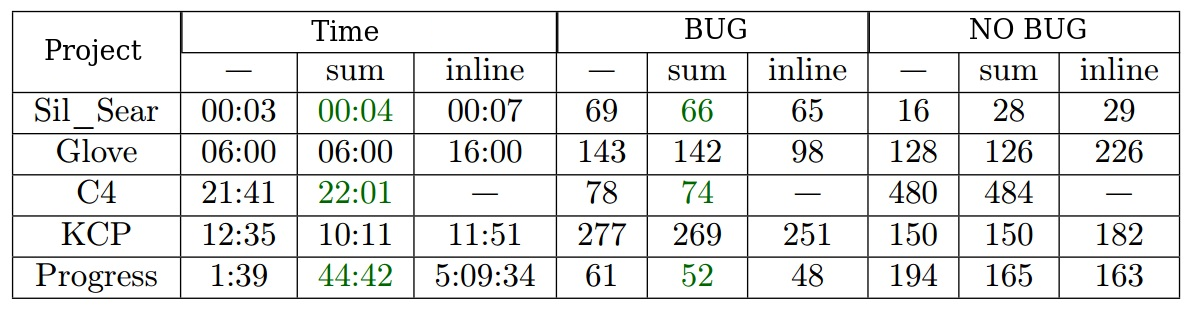
\includegraphics[keepaspectratio, width=\linewidth, height=8cm]{testing}
\end{table}

One can easily see from the evaluation results that the contract mining results are highly dependent on the analyzed project. If the project does not contain many mineable functions~(e.g., \texttt{wrk}), our algorithm shows little to no influence on the analysis results. On the other hand, if the project is big~(e.g., \texttt{git}), it will most probably contain a lot of different function calls, and we are able to collect a lot of interesting contracts.

\begin{table}[tbh]
\centering
\caption{Evaluation results}
\label{table:evaluation}

\begin{tabular}{|c|c|c|c|}
\hline
Project    & SLOC
           & Contracts \tablefootnote{number of collected contracts}
           & Violations\tablefootnote{number of contract violations found} \\ \hline
\texttt{beanstalkd} & 7.5k & 10  & 6 \\ \hline
\texttt{iputils}    & 12k  & 15  & 6 \\ \hline
\texttt{wrk}        & 80k  & 6   & 4 \\ \hline
\texttt{git}        & 340k & 186 & 59\\
\hline
\end{tabular}
\end{table}

Some examples of the extracted contracts for \texttt{git}, \texttt{iputils} and \texttt{beanstalkd} projects are shown in figure~\ref{fig:extracted-contracts}. Most of the contracts are pretty simple~(as we selected~$K$ and~$X$ with precision in mind) and may seem modest; but they were created in a fully automatic fashion and capture relevant safety preconditions, without any need for the user interaction. In our future work we plan to analyze the impact of the parameter selection on the extraction results in more detail.

\begin{figure*}[tbh]

\caption{Examples of the extracted contracts}
\label{fig:extracted-contracts}

\begin{lstlisting}[style=PS,multicols=2]
--- Project: git ---
--- Function: fgets ---
(@P (arg$2 == <nullptr>)=false)
--- Function: ungetc ---
(@P (arg$0 == 4294967295)=false)
--- Function: lseek64 ---
(@P (arg$0 < 0)=false)
--- Function: git_deflate_bound ---
(@P (arg$1 +> 1024)=true)
--- Function: get_next_line ---
(@P (arg$0 +< arg$1)=true)
--- Function: check_patch ---
(@P (arg$0 == <nullptr>)=false)
--- Function: write_branch_report ---
(
  @P (arg$1 == <nullptr>)=false,
  @P (arg$0 == <nullptr>)=false
)

--- Project: iputils ---
--- Function: ping4_run ---
(@P (arg$2 == <nullptr>)=false)
--- Function: ping6_run ---
(@P (arg$2 == <nullptr>)=false)
--- Function: probe_ttl ---
(@P (arg$0 < 0)=false)
--- Function: ioctl ---
(@P (arg$0 == 4294967295)=false)

--- Project: beanstalkd ---
--- Function readdir ---
(@P (arg$0 == <nullptr>)=false)
--- Function reply_job ---
(@P (arg$1 == <nullptr>)=false)
--- Function bind ---
(@P (arg$0 == 4294967295)=false)
--- Function store_job ---
(@P (arg$0 == <nullptr>)=false)

\end{lstlisting}
\end{figure*}
